\def\MWS{MathWebSearch\xspace}

In the \pn VRE toolkit approach, a virtual research environment (VRE) is based on software and data components (called D/K/S-bases in the original proposal) under a joint user interface.
Here we concentrate on a crucial aspect of this, the interaction of the D/K/S-base with the UI in mathematical Jupyter notebooks and interactive mathematical documents -- see ~\cite{ODK-D4.2} for a discussion of the concepts.
In particular, mathematical Notebooks allow users to navigate the combined information space of all the underlying tools, systems and resources integrated into the VRE as one. 
However, they aggravate the already serious problem of finding the piece of knowledge (or Notebook) a mathematician wants.
Of course, there is a text search engine built into  GitHub that can distinguish notebooks by file type, but as we well know, this only helps if the mathematician can already express her information through a bag of words.
When it comes to formulae, the GitHub search engine is essentially blind. 
Thus, we decided to adapt the \MWS formula search engine to this \pn joint user interface. 

\subsection{The \MWS Formula Search Engine}

\MWS is a web application that provides low-latency answers to full-text queries which consist of keywords and formulae.
We give only a brief overview of the pre-existing \MWS architecture here and refer the reader to~\cite{ProKoh:mwssofse12} and ~\cite{ODK-D6.1} for details. 
We furthermore describe our re-worked design in Section~\ref{sec:software:deployment} below.
In a nutshell, \MWS consists of a search web application (the \MWS daemon) that indexes formula harvests (essentially lists of content MathML formulae and URI references) and answers queries (Content MathML schemata with query variables).
Multiple domain-specific front-ends can talk to the \MWS daemon using an XML-based protocol, they transform the user's information into Content MathML queries. 

The \MWS system has been used to supply search instances on various corpora of mathematical documents, we describe two here, others can be seen on \url{http://search.mathweb.org}. 

\subsubsection{arXiv search}

Begun on August 14, 1991, created by Paul Ginsparg, the ``Cornell e-Print arXiv'' (\url{http://arXiv.org}) is a repository of scientific papers and electronic preprints in
fields of mathematics, computer science, physics, astronomy, biology and statistics or finance written in {\TeX/\LaTeX} for an optimized transfer over the internet and an easily rendered client-side.
In present the project is hosted by Cornell University and includes over a million articles and increases by around 8000 per month.

The KWARC group have converted the arXiv corpus into HTML5~\cite{StaKoh:tlcspx10} and harvested it for \MWS. The instance at \url{http://arxivsearch.mathweb.org}
indexes over 105\,000 math-heavy papers.
This subcorpus has also been used for the NTCIR Math Information Retrieval Challenges~\cite{AizKohOun:nmpto13,AizKohOunSch:nmto14,AizKohOunSch:nmto16}.

\subsubsection{zbMATH search}

Zentralblatt Math (zbMath) is a mathematical information service that curates a database of reviews and classifications (MSC, see~\cite{MSC2010}) for all articles in mathematics since the middle of the 19th century. The database currently contains 3.8 million reviews and grows at a rate of ca 120\,000 reviews per year.
The zbMATH portal at \url{https://zbmath.org/} offers a faceted search engine for reviews based on bibliographic metadata, MSC classification, and \emph{formulae}.
The latter is driven by \MWS. 

\subsection{Enabling Formula Search Deployments}\label{sec:software:deployment}

The previous \MWS deployments required a significant amount of application-specific code. 
This code was typically written by students, and as a result it was not of high quality. 
In particular, most code was too specialized to be re-usable. 

This made it impossible to directly use \MWS as part of the OpenDreamKit VRE Toolkit. 
To allow using \MWS flexibly, we needed to inject the system with a lot of software engineering. 
To achieve this, we developed new infrastructure on top of the core \MWS daemon. 
This works takes the form of several components, each of which can deployed independently using Docker (see also \WPref{component-architecture}).
The structure of our infrastructure can be seen in Figure~\ref{fig:mwsdeployment}, with new components in green. 

\begin{figure}[ht]
  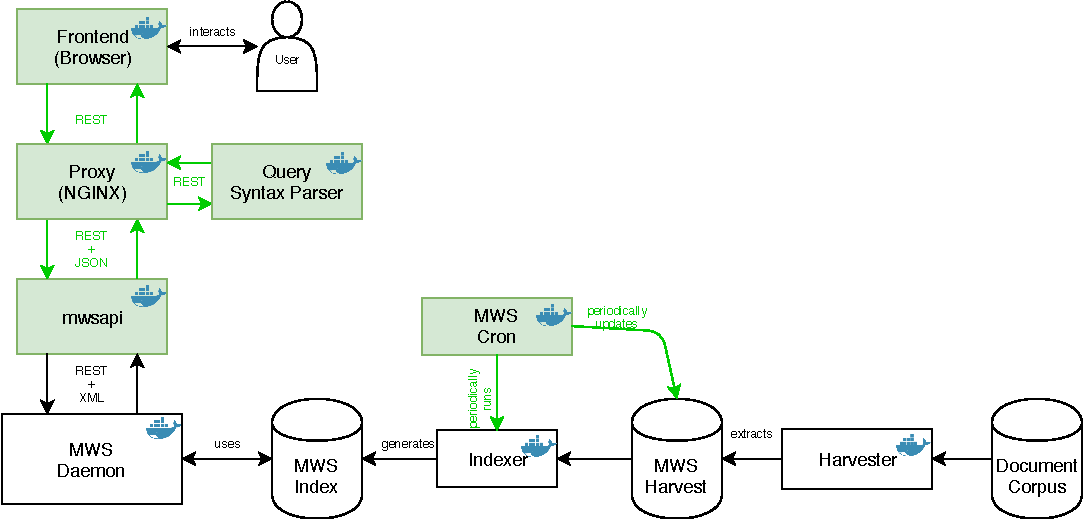
\includegraphics[width=1.0\textwidth]{mws_layout.pdf}
  \caption{Structure of our newly developed \MWS Deployment Infrastructure. Newly developed and updated components colored in green, components available as Docker Containers show the Docker logo.  }\label{fig:mwsdeployment}
\end{figure}

We describe the components of our infrastructure. 

\paragraph{The \MWS Daemon}
The central component is the \textit{\MWS daemon}, which can be found in the bottom left of Figure~\ref{fig:mwsdeployment}. 
As previously, it uses an \textit{Index} and exposes an XML-based API for queries. 
The only change we made to the core daemon is that it now exists inside a Docker Container at \cite{mwsdocker:on}.

\paragraph{The Harvesters and The Indexer}
As before, in order to generate an index from a set of documents we need two components. 
The indexer, as an application-independent component, has also been dockerized\cite{mwsindexer:github:on}. 
First we extract a set of ContentMathML formulae using a corpus-specific \textit{Harvester} (bottom right). 
The generated \textit{Harvest} is then sent to the \textit{Indexer} (bottom center), which generates or updates the \textit{Index}. 

Additionally, we introduced a new scheduler component called \textit{MWS cron}. 
This periodically sends updated harvests to the \textit{indexer}, which then in turn updates the index. 
This process ensures that the Index remains up-to-date, and does not have to be re-generated manually. 
The source code of this component can be found at \cite{mwscron:github:on}. 

The index consists of a set of highly optimized binary files. 
Usually, the index is stored on disk by the indexer, and then loaded into memory by the \MWS daemon when responding to queries. 
However, for small harvests a shortcut exists: the \MWS daemon can re-build an index every time it starts up and store it directly into memory, skipping the explicit indexing step. 
This enables us to extremely quickly deploy \MWS for small enough harvests. 
\paragraph{Frontend, mwsapi and the query syntax parser}

In order to process end user queries, we introduced several additional components.

The most important component of these is a new React-powered \textit{frontend} \cite{mwsfrontend:github:on}, which runs inside the users' browser or as a component of a web information system such as MathHub. 
It allows users to enter a formula search query and view the results. 
The frontend contains corpus-specific branding and text, but is otherwise not corpus-specific. 
In particular the querying code which interacts with the backend components, does not require specialization. 

While the \MWS daemon only understands formulae in Content MathML, users often enter them using different representations, such as \LaTeX. 
For this purpose, the frontend allows entering queries in human-writable, corpus-specific syntax. 
To transform the user query into a system-understood query, we make use of a new component called the \textit{Query Syntax Parser}. 
For {\LaTeX} syntax this is achieved using {\LaTeX}ML \cite{Miller:latexml:online} along with a custom \MWS extension for it\cite{latexml-stex:github:on}, but this component is fully interchangeable if the user desires other syntaxes. 

The frontend does not directly send MathML queries to the \textit{Daemon}.
Instead, it sends them to a thin API layer on top called \textit{mwsapi}. 
This layer forwards the queries to the daemon and, upon receiving a response, performs some post-processing. 
This process includes transforming substitutions returned by \MWS into a format that can be directly presented to the user by the frontend. 
The layer is written in go and doubles as api bindings to use MathWebSearch programatically in other applications. 
The source code and documentation are available on Github at \cite{mwsapi:github:on}. 

As the frontend, the mwsapi server and the Query Syntax Presenter are all exposed to the end-user under the same url, a proxy delegating requests accordingly was also necessary. 
This is using an nginx server. 

\subsection{Building a SageMath Notebook Search Application}

SageMath can produce \LaTeX\ formulae as output. 
Recall that mathematical Notebooks allow users to navigate the combined information space of all the underlying tools, systems and resources integrated into the VRE as one. 
These formulae are part of this combined information space, and are something that mathematicians want to search for.
Using the newly developed infrastructure above, it was straightforward to apply \MWS and enable users to perform such searches. 

Applying our infrastructure involved several steps, which we briefly describe below.

\paragraph{Harvesting Formulae}
To enable \MWS to search the formulae, we needed to build a harvester that extracted formulae from a notebook and as ContentMathML formulae. 
To achieve this, we converted each \LaTeX\ formula via LaTeXML and aggregated them inside an \MWS Harvest file. 
The script to achieve this can be found at \cite{mwsjupyterharvest:github:on} and involved around 100 lines of straightforward Python script written in a few hours. 

To test our harvester, we decided to make use of Sage Jupyter Notebooks found on GitHub. 
We implemented a second Python script which used the GitHub API to download all matching files and then apply our harvester to them. 
There are approximately $10000$ matching SageMath notebooks on GitHub, totalling to approximatly $5800000$ expressions\footnote{An expression is a \MWS-indexed subterm of a formula. }. 
\paragraph{Query Syntax Parser}

To enable users to search the formulae in an appropriate syntax, a query syntax parser was required. 
However, as Sage produces \LaTeX\ formulae, we can re-use the {\LaTeX}ML query syntax parser for this purpose. 

\paragraph{Deploying the system}

The third and final step involved deploying the system.
This consisted of deploying the various involved Docker Containers. 
For this purpose we made use of a tool called Docker Compose~\cite{docker-compose:on}. 
Docker Compose allows defining complex interactions between containers in a simple docker compose file. 
The tool then automatically starts containers as described in this file. 
For our \MWS application we only needed to adapt a generic \MWS Docker-Compose file with the public website URL and appropriate branding for the frontend. 

\begin{figure}[ht]
  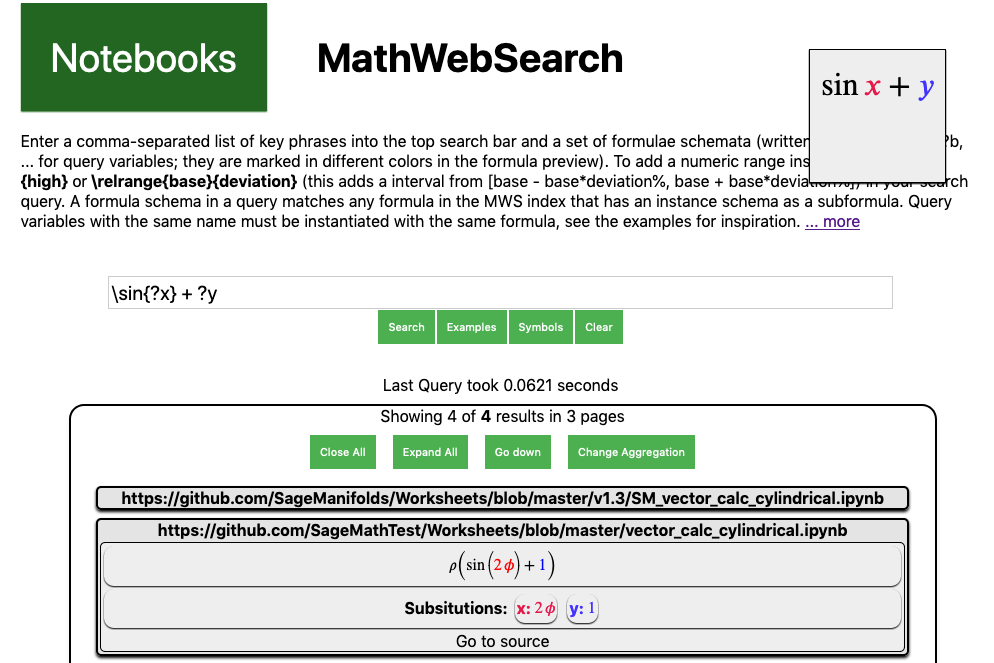
\includegraphics[width=\textwidth]{mwsnotebookfront.png}
  \caption{The deployed Jupyter Notebook Search Frontend}\label{fig:mwsnotebookfront}
\end{figure}

The user interface is deployed at \url{https://jupytersearch.mathweb.org} and can be seen in Figure~\ref{fig:mwsnotebookfront}.
To perform a search, users first enter a formula with query variables to search for in the central search box. 
In this case the query $\sin{x} + y$ was entered and $x$ and $y$ were marked as query variables by prefixing them with a ?. 
Next, the search query was rendered by {\LaTeX}ML, which can be seen in the top right. 
To then view the search results users had to click the green search button. 
This caused the query to be sent to \MWS. 

The results of the query can then be seen in the bottom half of the image.
In this case, the query took $0.0621$ seconds and returned $4$ results. 
To not clutter the page with too many details, results can be expanded individually. 
In this case, the user choose to only expand one particular result. 
For this result, several details can be seen -- the url of the notebook it was found in, the matching formula, and the subsituted query variables. 
The query variables are colored for easy visibility -- here $x$ matched the term $2\Phi$ and is colored red and $y$ matched the term $1$ and is colored blue. 

In addition the notebook search, we have also exercised a similar progress for the $n$-category Cafe (nLab, \url{https://ncatlab.org/}, a community-run semantic wiki on category theory and applications with more than 13K pages). 
Similar to notebooks, NLab also contains formulae in \LaTeX\ syntax, enabling us to largely re-use all components we had created previously.  The NLab Harvester can be found at \cite{nlabharvester:github:on}, and the corresponding frontend at \url{https://nlabsearch.mathweb.org}.

%%% Local Variables:
%%% mode: latex
%%% mode: visual-line
%%% fill-column: 5000
%%% TeX-master: "report"
%%% End:

%  LocalWords:  ednote textbf fig:mwsdeployment includegraphics textwidth mws_layout.pdf textit mwsapi specialization nginx Jupyter customized evalutation temasearch xspace newpart standardized ProKoh:mwssofse12 subsubsection Ginsparg optimized StaKoh:tlcspx10 AizKohOun:nmpto13,AizKohOunSch:nmto14,AizKohOunSch:nmto16 zbMATH emph specialized WPref colored dockerized customization NLab oldpart mwsnotebookfront.png fig:mwsnotebookfront
